\section{Example of CFPQ With Combinators}\label{sect:combinators}

In this section we demonstrate the main features of combinators in the context of context-free path querying and integration with general-purpose programming languages.
We first introduce a simple graph analysis problem and then show how to solve it by using parser combinators.
In our work we use the combinators library Meerkat.Graph~\footnote{Meerkat.Graph repository: \url{https://github.com/yaccconstructor/meerkat}. Access date: 12.03.2020}.

\underline{\textbf{Problem statement.}}
Suppose we have an RDF graph and want to analyze hierarchical dependencies over different types of relations.
Our goal is, for the given object, to find all objects which lie on the same level of the hierarchy.
Namely, for the given set of relations $r = \{R_0 \ldots R_i\}$ and for the given vertex $v$ we want to find all vertices reachable from $v$ by paths which specified by the following context-free grammar in EBNF:
%\begin{align*}
 %\textit{qSameGen} \to & {R_0}^{-1} R_0 \mid \ldots {R_i}^{-1} R_i  \mid \\
 %                      & {R_0}^{-1} \textit{qSameGen } R_0 \mid \ldots \mid {R_i}^{-1} \textit{qSameGen } R_i.
 $\textit{qSameGen} \to {R_0}^{-1} \textit{qSameGen? } R_0 \mid \ldots \mid {R_i}^{-1} \textit{qSameGen? } R_i.$
 %\end{align*}
Additionally, we want to calculate the length of these paths.

%\subsection{Simple Solution}

The first step is to specify a paths constraint.
For example, we consider relation to be \verb|skos__narrowerTransitive|.
Then constraint may be specified in terms of combinators as follows:

\begin{lstlisting}
val rName = "skos__narrowerTransitive"
def qSameGen () =
    syn(inE((_: Entity).label() == rName) ~ qSameGen().? ~
        outE((_: Entity).label() == rName))
\end{lstlisting}

Here we use \verb|inE| and \verb|outE| to specify the incoming and outgoing edges with the respective labels, \verb|~| to concatenate subqueries, and \verb|.?| to specify an optional subquery.

This query specifies exactly the path wanted, but is still not a solution.
First of all, we cannot specify start vertex and cannot extract final vertices.
Also, this query is for a single relation.
To investigate hierarchy over a set of relations we need to rewrite it.

\underline{\textbf{Compositionality.}}
The first step is to generalize the query to simplify the handling of different types of relations.
We introduce a helper function \verb|reduceChoice| which takes a list of subqueries and combines them using the alternation operation.

\begin{lstlisting}
def reduceChoice(qs: List[_]) =
  qs match {
     case x :: Nil => x
     case x :: y :: qs => syn(qs.foldLeft(x | y)(_ | _))
  }
\end{lstlisting}

After that, we use this function in the new version of \verb|sameGen| to combine subqueries for different types of ``brackets''.
The brackets are passed as parameters so the query can be instantiated for different brackets.

\begin{lstlisting}
def sameGen(brs: List[(_,_)]) =
    reduceChoice( brs.map {
      case (lbr, rbr) => syn(lbr ~ sameGen(brs).? ~ rbr)
      })
\end{lstlisting}

Now we are ready to specify the start vertex and to collect final vertices.
First of all, we provide a filter to select only vertices with \verb|uri| property.

\begin{lstlisting}
val uriV = syn(V((_: Entity).hasProperty("uri")) ^^)
\end{lstlisting}

We create a function \verb|queryFromV| which takes the start vertex \verb|startV| and a path \verb|query| as an input, and creates a query to find all vertices with \verb|uri| property which are reachable from the \verb|startV| by a path from the \verb|query| result.
Finally, we collect values of \verb|uri| for all reachable vertices by specifying a user-defined action {\small \verb|{case _ ~ _ ~ (v: Entity) => v.getProperty[String]("uri")}|} which captures the result of query (it is a triple-sequence of subqueries results) and gets the \verb|uri| property from the result of the last subquery.

\begin{lstlisting}
def queryFromV (startV, query) =
  syn(startV ~ query ~ uriV &
      {case _ ~ _ ~ (v: Entity) =>
            v.getProperty[String]("uri")})
\end{lstlisting}


\underline{\textbf{User-defined actions.}}
The final step is to extend the query to calculate lengths of all paths which satisfy conditions.
To do this, we equip \verb|sameGen| with additional user-defined actions.

\begin{lstlisting}
def sameGen(brs: List[(_,_)]) =
    reduceChoice(
      brs.map {
        case (lbr, rbr) =>
          syn((lbr ~ (sameGen(brs).?) ~ rbr) & {
            case _~Nil~_ => 2
            case _~((x:Int)::Nil)~_ =>  x + 2
          })})
\end{lstlisting}

The \verb|queryFromV| now also handles the second element of the triple in order to get access to the accumulated lengths.

\begin{lstlisting}
def queryFromV(startV, query) =
    syn(startV ~ query ~ uriV &
      {case _ ~ (len:Int) ~ (v:Entity) =>
        (len, v.getProperty[String]("uri"))})
\end{lstlisting}

Now we are ready to combine the functions and evaluate the query.
First, we add a helper function \verb|makeBrs| which takes a list of relation names and creates a list of pairs of subqueries which check incoming and outgoing edges respectively (pairs of brackets).

\begin{lstlisting}
def makeBrs (brs:List[_]) =
    brs.map(name =>
       (syn(inE((_: Entity).label() == name) ^^),
        syn(outE((_: Entity).label() == name) ^^)))
    .toList
\end{lstlisting}

The main function \verb|runExample| takes a list of relations, the start vertex and the graph, builds the same generation query over the given relations by using the functions described and executes it.

\begin{lstlisting}
def runExample (brs: List[_], startVId, graph) =
    val startV = V(getIdFromNode(_: Entity) == startVId
    executeQuery(queryFromV( syn(startV)^^),
                               sameGen(makeBrs(brs))),
                   graph).toList
\end{lstlisting}

To execute the query for the vertex 1, one should call \verb|runExample| as presented below.

\begin{lstlisting}
runExample(RDFS__SUB_CLASS_OF :: Nil, 1, graph)
\end{lstlisting}

\underline{\textbf{Type safety.}}
As far as queries are functions of a general-purpose language, which is used to develop the application, its compiler type checks the queries and their results statically.

Figure~\ref{fig:types} demonstrates the example of type checking.
There is an error in the way the total length of the paths is computed: the indentifiers of the final vertices are summed instead of the lengths.
The~compiler statically detects a type error because an integer is expected but a string is provided.

\begin{figure}[ht]
   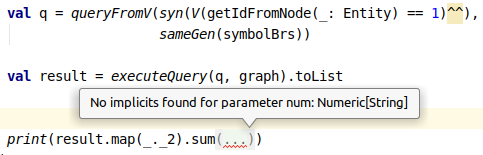
\includegraphics[width=0.48\textwidth]{pictures/image.png}
   \vspace{-0.2cm}
   \caption{Error notification in a query in IntelliJ IDEA}
   \label{fig:types}
\end{figure}

\underline{\textbf{IDE Support.}}
By using an IDE to write queries, one can benefit from such features as syntax highlighting, code navigation, autocompletion without any additional effort.
Figure~\ref{fig:autocompletion} shows an example of autocompletion suggestion for a vertex.

\begin{figure}[ht]
    \centering
    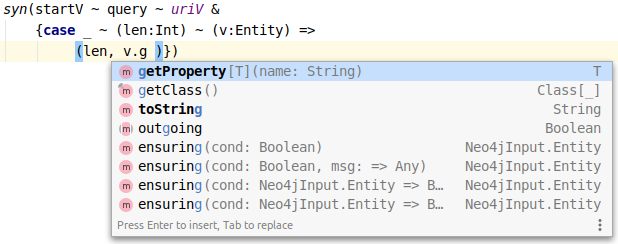
\includegraphics[width=0.48\textwidth]{pictures/image1.png}
    \caption{Query auto-completion in IntelliJ IDEA}
    \label{fig:autocompletion}
\end{figure}
